%%% Ejemplo de Paper para JNIC 206

\newcommand{\CLASSINPUTinnersidemargin}{18mm}
\newcommand{\CLASSINPUToutersidemargin}{12mm}
\newcommand{\CLASSINPUTtoptextmargin}{20mm}
\newcommand{\CLASSINPUTbottomtextmargin}{25mm}
\documentclass[10pt,conference,a4paper]{IEEEtran}
%%%%%%%%%%%%%%%%%%%%%%%%%%%%%%%%%%%%%%%%%%%%%%%%%%%%%%%%%%%%%%%%%%%%%%%%%%%%%%%%%

%%% Tildes y demás caracteres en castellano...
%\usepackage[latin1]{inputenc}
% o bien
\usepackage[utf8]{inputenc}


%%% Fuente Times...
\usepackage{times}


%%% Figuras en formato .png, .ps, pdf o eps
\usepackage{graphicx}
\usepackage{subfigure}
\DeclareGraphicsExtensions{.png,.eps,.ps,.pdf}

%%% Formato y tipografía de URL, direcciones de correo...
\usepackage{url}
\usepackage{amsmath}
% Hyperlinks for clickable IEEE-style citations.
% Load after most packages; keep links unobtrusive.
\usepackage[hidelinks]{hyperref}

%%% Sección para definir explícitamente la separación de sílabas al final de una línea:
\hyphenation{si-guien-do}

%%% Secciones etc. en castellano
\usepackage[english]{babel}

\sloppy

\begin{document}

%%% Título
% --- Project title (active) ---
\title{Zaguik: Zero-Knowledge Attestation for Privacy-Preserving LLM Governance}
%
% --- Template title kept for reference (disabled) ---
\iffalse
\title{Ejemplo de trabajo para XI JNIC. Siga las instrucciones proporcionadas, indicando el tipo de trabajo de que se trata}
\fi


%%% Autores
\author{\IEEEauthorblockN{Jan Aguiló Plana}
\IEEEauthorblockA{Universitat Pompeu Fabra\\
Carrer de Roc Boronat, 138, Barcelona\\
jan.aguilo01@estudiant.upf.edu}
\and
\IEEEauthorblockN{Vanesa Daza}
\IEEEauthorblockA{Universitat Pompeu Fabra\\
Carrer de Roc Boronat, 138, Barcelona\\
vanesa.daza@upf.edu}}


\maketitle


%%% Resumen
\begin{abstract}
Regulators increasingly require evidence-backed assurances about how AI systems
handle sensitive information. We present Zaguik, a privacy-preserving attestation
pipeline that proves, in zero knowledge, that a large language model (LLM)
response passed a personally identifiable information (PII) filter, without
revealing either the response text or the filtering model. The system generates
an LLM response, applies a PII detection policy, and produces a
zk-SNARK using EzKL over the detector inference. The proof exposes only a
public commitment (a hash) to the exact response, binding verification to the
delivered output while keeping its contents private; filtering logic and outputs remain private. We provide a runnable reference
implementation, discuss practical setup requirements and ONNX compatibility constraints, and outline how such
proofs can support GDPR-aligned auditing and transparent AI governance.
\end{abstract}
%
% --- Template abstract kept for reference (disabled; do not delete) ---
\iffalse
\begin{abstract}
  Este documento constituye la plantilla para las {\it X Jornadas
    Nacionales de Investigación en Ciberseguridad} (JNIC 2026), organizadas
  por la Universitat Politècnica de Catalunya.
  El {\it abstract} debe contener entre 100 y 150 palabras.
  El tipo de letra es {\it Times New Roman negrita, 9 ptos.}, tal y
  como aparece en esta plantilla. Se recomienda no emplear acrónimos en esta
  sección. Esta plantilla ha sido generada tomando como base el estándar de
  documentos IEEE~\footnote{Disponible para \LaTeX, como plantilla de estilo
    \texttt{IEEEtran.cls}.}. Por favor, utilice esta plantilla como formato
  base para su trabajo. Para más información sobre la organización y
  desarrollo de las jornadas, consulte el enlace \url{https://www.incibe.es/eventos/JNIC/JNIC2026}.
\end{abstract}
\fi


%%% Palabras clave
%\begin{IEEEkeywords}
%Jornadas, Ciberseguridad
%\end{IEEEkeywords}


%%% Tipo de contribución: seleccione lo que proceda, eliminando el resto del texto
%{\bf Tipo de contribución:}  {\it Investigación en desarrollo}


%%% Introduction
\section{Introduction}

Artificial intelligence (AI) systems that process personal data are increasingly subject to enforceable obligations beyond voluntary transparency pledges. Regulations such as the European Union's General Data Protection Regulation (GDPR) and emerging AI acts require evidence-backed assurances about how systems handle sensitive information, comply with safety requirements, and respect data-subject rights. For large language models (LLMs) deployed in customer-facing or regulated settings, demonstrating that outputs do not leak personally identifiable information (PII) is both a legal necessity and a trust requirement. Auditors and regulators need not only policies on paper but verifiable guarantees that those policies are actually applied in production.

Today, verifying that a provider applies a PII filter to LLM outputs typically requires the auditor to trust the provider's claims or to inspect the outputs and the filtering logic directly. If the auditor sees the raw outputs, privacy is compromised; if the provider must disclose the filtering model or its parameters, intellectual property and competitive concerns arise. This tension leaves a gap: there is no cryptographically sound way to prove that a given output was filtered for PII without revealing either the output or the internals of the filter. Zero-knowledge proofs (ZKPs) address this need by allowing one party (the prover) to convince another (the verifier) that a statement is true without revealing the underlying data or computation. Applied to AI pipelines, ZKPs can attest that a specific computation was performed (e.g., that a PII filter was applied and that its result indicated no PII) while keeping the model and the actual text private.

In this work we describe and implement Zaguik, a system that produces such a verifiable, privacy-preserving attestation for LLM outputs. The pipeline works as follows: (1) an LLM generates a response to a user prompt; (2) a PII filter (in our reference implementation, a regex-based detector) is applied to the output; (3) if the output passes the filter, a SHA256 hash of the output is computed and the output is encoded as input to a circuit; (4) a zk-SNARK proof is generated using EzKL, attesting that the filter was applied and that the circuit output corresponds to a ``clean'' result, with the proof bound to the hash of the response; (5) any verifier holding the hash and the proof can confirm that filtering was correctly applied without ever seeing the text or the filter internals. The proof thus ties verification to the exact delivered output while preserving confidentiality. This approach illustrates how cryptographic attestation can support transparent AI governance: compliance and audit can be based on verifiable proofs rather than on trust alone, and both user privacy and provider confidentiality can be preserved. We provide a runnable reference implementation and discuss practical considerations.


\section{Related Work}
% Body to be completed.
\subsection{Zero-Knowledge Proof Systems}

Zero-knowledge proof systems such as Groth16~\cite{groth2016size}, PLONK~\cite{gabizon2019plonk}; and related zk-SNARK constructions provide succinct and efficiently verifiable proofs of correct computation over arithmetic circuits. These systems allow a prover to convince a verifier that a computation was executed correctly without revealing private inputs.

More recently, practical toolchains such as libsnark~\cite{bensasson2014vn}, Halo2, and EzKL have enabled developers to compile high-level programs and machine learning models into circuits suitable for zk-SNARK proving.

However, these works focus on the cryptographic machinery for proving circuit execution correctness. They do not address the governance question of how such proofs can be used to attest enforcement of content filtering policies over LLM outputs without revealing those outputs.

\subsection{Zero-Knowledge Machine Learning (ZKML)}

Zero-knowledge machine learning focuses on proving correct execution of machine learning inference without revealing private inputs. zkCNN~\cite{liu2021zkcnn} demonstrates how convolutional neural network predictions and accuracy can be verified in zero knowledge by expressing inference as arithmetic circuits. Similarly, vCNN~\cite{lee2024vcnn} presents a framework for generating zk-SNARK proofs that certify correct execution of convolutional neural network inference.

These works address inference correctness: proving that a model’s output was computed faithfully according to fixed parameters. In contrast, our work does not aim to prove correct execution of the LLM itself. Instead, we focus on attesting enforcement of a post-generation filtering policy over LLM outputs. To our knowledge, prior ZKML research does not address governance-level attestation of output filtering for generative models, where the goal is not to prove the model computation but to prove that a compliance constraint was applied to the generated output.

\subsection{Privacy-Preserving Machine Learning and Inference}

Research in privacy-preserving machine learning includes techniques such as secure multiparty computation~\cite{lindell2009smpc}, homomorphic encryption for neural network inference~\cite{gilad2016cryptonets,brutzkus2019lowlatency}, and confidential computing enclaves.

These approaches focus on protecting either model parameters or user inputs during inference. For example, homomorphic encryption allows inference over encrypted data without revealing the input, while secure multiparty computation distributes trust across multiple parties.

Our work differs in focus: rather than protecting model inputs or parameters, we aim to protect the model output while still enabling verifiable policy enforcement. The output remains private, yet a verifier can be assured that a specified constraint was checked.

\subsection{AI Auditing, Transparency, and Governance}

AI governance frameworks emphasize auditing, transparency, and accountability. Model cards~\cite{mitchell2019modelcards}, datasheets for datasets~\cite{gebru2018datasheets}, and regulatory frameworks such as the EU AI Act propose documentation-based or process-based accountability.

In practice, auditing of deployed systems typically requires access to logs, outputs, or internal documentation. Such approaches rely on institutional trust and do not provide cryptographic guarantees of enforcement at runtime.

Recent discussions in AI safety research have proposed verifiable AI or cryptographic attestation mechanisms, but concrete implementations for generative output filtering remain limited.

Our work contributes a concrete mechanism for cryptographically attesting that a filtering policy was executed on a specific LLM output, without revealing that output to the verifier.

\subsection{PII Detection and Content Moderation}

Personal data detection is commonly performed using rule-based systems (regex patterns), named entity recognition models, or hybrid approaches~\cite{dernoncourt2017deid}. Production systems for content moderation rely on deterministic filters, ML classifiers, and policy enforcement pipelines.

However, these systems provide enforcement but not verifiability. An external auditor must either trust the system operator or inspect outputs directly. To our knowledge, prior work on PII filtering does not provide a mechanism for cryptographically proving that filtering was applied to a given output without revealing the output itself.

\subsection{Positioning Statement}

To our knowledge, no prior work combines zero-knowledge proofs with LLM output filtering to provide privacy-preserving attestation of policy enforcement. Existing zk-SNARK and ZKML systems enable proving correct circuit execution, but they do not address governance-level questions of output compliance. Conversely, AI auditing and moderation systems enforce policies but lack cryptographic verifiability.

Our work occupies the intersection of these domains: we demonstrate a practical prototype that attests enforcement of an output constraint over LLM-generated text while preserving output confidentiality.

\section{Methodology}
\label{sec:methodology}

The core contribution of this work is the \emph{cryptographic attestation pipeline}: we show how to produce a zk-SNARK proof that a given string was passed through a certified check, with the proof bound to a commitment to the output and with no disclosure of the text or the checker's internals. The PII filter is the policy we attest to; its design is deliberately simple so that the focus remains on the proof system. Below we describe the architecture, the filter used in the current implementation, the encoding of outputs for the circuit, the proof system and visibility semantics, and the setup, proof, and verification procedures.

\subsection{System Overview}

The pipeline has two phases: a \emph{filtering phase} and a \emph{proof phase}. In the filtering phase, a user prompt is answered by an LLM (in our implementation we use DistilGPT-2); the response is then checked by a PII detector. Only if the detector reports that the text contains no PII do we enter the proof phase. There we encode the (clean) output as input to a circuit that models the same filtering logic, generate a zk-SNARK proof over that circuit using EzKL, and output a proof bound to a public commitment (hash) of the response. A verifier who receives the proof and the commitment can check that the filtering computation was correctly applied to the committed output, without learning the text or the internal parameters of the filter. The LLM itself is out of scope of the proof: we attest only that a given string was passed through the certified PII filter and passed.

\begin{figure}[htbp]
	\centering
	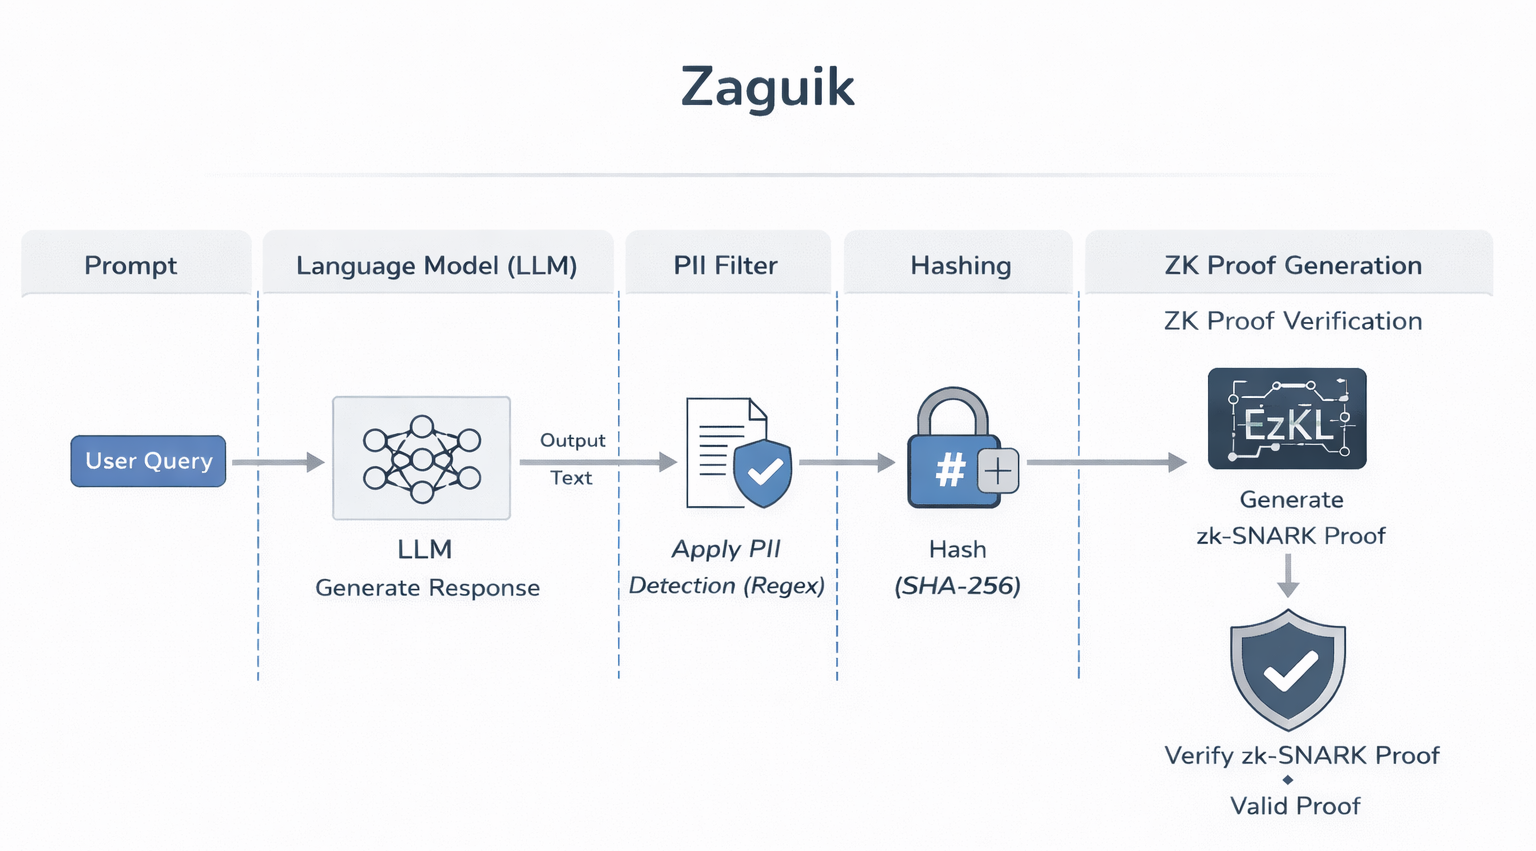
\includegraphics[width=\columnwidth]{system_overview.png}
	\caption{Zaguik's end-to-end workflow: from user prompt and LLM response through PII filtering to proof generation and verification.}
	\label{fig:system_overview}
\end{figure}

\subsection{Formal Statement and Security Model}

We formally define the statement that Zaguik proves and clarify the visibility of data in the zero-knowledge setting.

\paragraph{Notation.}
Let $y \in \{0,1\}^*$ denote the output string generated by the LLM.  
Let $H(\cdot)$ be a cryptographic hash function (SHA256 in our implementation).  
Let $F$ denote the PII filtering policy.  
Let $C$ be the certified arithmetic circuit that implements $F$.  
Let $L$ be the fixed input length in bytes used for encoding (in our implementation $L = 2048$).  
Let $\mathrm{Enc}_L(y)$ denote the byte-level encoding of $y$, truncated or zero-padded to length $L$.

\paragraph{Public and Private Data.}
The zero-knowledge proof distinguishes between public inputs and private witness:

\begin{itemize}
    \item \textbf{Public input:}
    \begin{itemize}
        \item $h = H(y)$, a commitment to the LLM output.
        \item The verification key associated with circuit $C$.
    \end{itemize}
    \item \textbf{Private witness:}
    \begin{itemize}
        \item The full LLM output string $y$.
        \item Its encoded representation $x = \mathrm{Enc}_L(y)$.
        \item The internal witness values required to execute circuit $C$.
    \end{itemize}
\end{itemize}

The verifier learns only the commitment $h$ and the proof. The underlying text $y$ and the internal circuit execution remain hidden.

\paragraph{Language Definition.}
The proof system attests membership in the following NP language:

\[
\mathcal{L} = \{\, h \mid \exists y \text{ such that } H(y)=h \land C(\mathrm{Enc}_L(y)) = 1 \,\}.
\]

In other words, $\mathcal{L}$ contains all hash values for which there exists a corresponding text that both matches the hash and passes the certified PII filtering circuit.

\paragraph{Zero-Knowledge Statement.}
The prover demonstrates, in zero knowledge, that:

\[
\exists y \text{ such that } H(y)=h \land C(\mathrm{Enc}_L(y)) = 1.
\]

Informally, this means:

\begin{quote}
``There exists an LLM output $y$ that corresponds to the public hash $h$, and when processed by the certified PII filtering circuit $C$, the result is \texttt{PASS}.''
\end{quote}

In our current implementation, the consistency between the public hash $h$ and the encoded input $\mathrm{Enc}_L(y)$ is enforced at the protocol level: the prover computes both values from the same output string prior to proof generation. The hash equality is not verified inside the arithmetic circuit.

\paragraph{Scope of the Guarantee.}
The proof guarantees correct execution of the certified filtering circuit on the committed output. It does not guarantee that the filtering policy is complete or semantically sufficient, nor does it make claims about the internal behavior of the LLM. The guarantee is limited to enforcement integrity: that the specific circuit $C$ was correctly executed on a text consistent with the public commitment.

\subsection{PII Filtering and Policy}

We distinguish clearly between two components of the filtering pipeline: an operational PII detector used in plain execution, and a circuit-friendly policy used for zero-knowledge attestation.

First, the system applies a regex-based PII filter in plain execution. This detector searches for structured patterns such as email addresses, phone numbers, identification numbers, and other commonly formatted personal data. Its role is operational: it acts as a gating mechanism, preventing obviously unsafe outputs from proceeding to the proof generation stage.

Second, for zero-knowledge attestation, we implement a separate, circuit-friendly policy as a small PyTorch module that is exported to ONNX and compiled into an arithmetic circuit using EzKL. This module operates at the byte level. It takes as input a fixed-length normalized byte vector and counts occurrences of selected “suspicious” byte values (e.g., '@', '-', '.', and digits). The circuit outputs a scalar count, and the policy is considered satisfied if this count is zero.

The zk-SNARK proof certifies correct execution of this ONNX-derived byte-level circuit and the fact that its output equals zero. It does not certify direct execution of the plain regex filter. The regex detector and the byte-counter circuit are separate mechanisms: the former provides practical PII detection in deployment, while the latter encodes a structurally checkable constraint that can be efficiently represented and verified within an arithmetic circuit.

It is therefore important to clarify the scope of equivalence. The proof guarantees only that the ONNX circuit was executed correctly on the encoded output. The correspondence between the plain regex-based filter and the byte-level circuit is a design choice, not a formally verified equivalence. The byte-counter policy can be interpreted as a conservative structural proxy for certain classes of PII indicators, but it does not capture the full semantic expressiveness of the regex detector. Establishing formal semantic equivalence between high-level filtering logic and its circuit representation remains an open research problem and is outside the scope of this prototype.

The attestation mechanism itself is policy-agnostic: any deterministic filtering rule that can be expressed as an ONNX model compatible with the proof backend can be certified in the same manner. In this work, the simplified byte-level policy serves to demonstrate the feasibility of zero-knowledge attestation for LLM output governance under current practical constraints.
\subsection{Encoding and Circuit Input}

The LLM output is a string. To feed it into the circuit we encode it in fixed-size form. We fix an upper bound L on the number of UTF-8 bytes (in our implementation L = 2048). The LLM generation process is configured so that attested outputs do not exceed L bytes. Therefore, for every attested output, the circuit receives the entire string.

We use a byte-level encoding: the UTF-8 representation of the string is zero-padded to length L if shorter. Each byte is normalized to [0,1] by dividing by 255. The resulting vector has shape [1, L] and is used as the single input tensor to the ONNX circuit.

The same string that passes the plain PII check is encoded and provided as private witness input to the circuit. The circuit operates over this full encoded representation.

Separately, we compute a SHA256 hash of the complete output string. This hash serves as a public commitment that binds the proof to the exact delivered response. The hash is not used as circuit input; instead, it is provided as public data alongside the proof so that external parties can associate the attestation with a specific output.
\subsection{Proof System and Visibility Semantics}

We use EzKL to compile the ONNX model into an arithmetic circuit and to produce zk-SNARK proofs (succinct, non-interactive arguments of knowledge). The security and privacy guarantees depend on how inputs, outputs, and parameters are exposed.

The encoded \emph{input} is kept private as witness data. The verifier learns only the zk-SNARK proof and the public hash commitment: the prover commits to the encoded output string, and the verifier learns this commitment but not the underlying bytes, so the LLM response stays private while the proof is bound to a specific output. The \emph{output} of the circuit is made available to the verifier so they can check that it indicates ``pass'' (e.g., zero PII score). The filter \emph{parameters} are fixed in the circuit and not revealed; the verifier only learns that the same certified circuit was executed. Together, these choices ensure that we prove ``this committed output was run through the certified PII filter and passed'' without leaking the text or the filter internals.

\subsection{Setup and Proof Generation}

Setup is performed once per circuit (e.g., per ONNX model and settings). The ONNX is used to generate the proof-system settings and to compile an arithmetic circuit; a KZG structured reference string (SRS) is required and can be obtained from a trusted source or generated locally for testing. With the compiled circuit and SRS, key generation yields a proving key and a verification key.

For each clean LLM output we wish to attest, we encode it as input data, compute the witness for the circuit, and run the prover to produce the final proof. The proof, the verification key, and (in deployment) the public commitment to the output are what the verifier needs.

\subsection{Verification}

Verification is deterministic: given the proof, the verification key, the settings, and the SRS, the verifier runs the verification algorithm and accepts if and only if the proof is valid. No secret data is required. If the verifier holds a hash of the LLM output (e.g., SHA256 or the in-circuit commitment), they can confirm that the proof applies to that exact output, so that attestation is non-detachable and binding.

\subsection{Implementation and Reproducibility}

Our reference implementation is in Python. The PII filter is regex-based in the current experiments. The cryptographic pipeline (regex-derived ONNX export, encoding, setup, proof generation, and verification) is implemented as a single scriptable workflow. The default configuration builds the small regex-derived ONNX, runs setup, and then generates and verifies proofs for a given text string. All steps are documented so that the pipeline can be reproduced and extended; integrating a more expressive PII model would require an ONNX export that is compatible with the proof system backend.

\section{Results}

We evaluate the full pipeline consisting of LLM generation, byte-level encoding, ONNX circuit execution, proof generation, and verification. Experiments were conducted using three independent prompts. Each prompt was designed to produce a long output exceeding 2048 bytes in order to evaluate different circuit encoding sizes $L$. For each output, the pipeline was executed with \[L \in \{128, 256, 512, 1024, 2048\}.\]
When $L < 2048$, only the prefix of length $L$ bytes was encoded and attested. Reported metrics in Table~II correspond to the mean over the three runs.

Table~I reports the one-time setup costs for the circuit with $L = 2048$. This includes settings generation, circuit compilation, structured reference string (SRS) generation, witness setup, and key generation. The total setup time was 102.44 seconds. SRS generation required 77.88 seconds, and key generation required 23.77 seconds. The remaining steps each took less than one second.

\begin{table}[htbp]
\centering
\caption{One-time setup costs (regex PII ONNX, $L=2048$).}
\label{tab:setup}
\begin{tabular}{l r}
\hline
\hline
Step & Time (s) \\
\hline
Settings generation & 0.14 \\
Circuit compilation & 0.02 \\
SRS generation$^{a}$ & 77.88 \\
Witness (setup) & 0.63 \\
Key generation & 23.77 \\
\hline
Total & 102.44 \\
\hline
\hline
\multicolumn{2}{l}{\small $^{a}$Generated locally for testing; production deployments would} \\
\multicolumn{2}{l}{\small download the SRS from a trusted source.} \\
\end{tabular}
\end{table}

Table~II presents proof size, proof generation time, witness computation time, and verification time for different values of $L$.

\begin{table}[htbp]
\centering
\caption{Proof size and timings vs.\ circuit encoding size $L$ (mean over 3 independent runs; reference output = 2048 bytes, prefix-truncated for $L < 2048$).}
\label{tab:results}
\begin{tabular}{c r r r r}
\hline
\hline
$L$ (bytes) & Proof size & Proof gen. & Witness & Verify \\
  & (bytes) & (ms) & (ms) & (ms) \\
\hline
128  & 21882.33 & 15982.16 &  71.07 & 204.29 \\
256  & 21861.33 & 12808.53 & 145.18 & 184.43 \\
512  & 21921.67 & 13796.08 & 154.59 & 172.77 \\
1024 & 21924.00 & 14408.21 & 318.23 & 171.83 \\
2048 & 21903.67 & 16142.74 & 529.71 & 172.20 \\
\hline
\hline
\end{tabular}
\end{table}

Proof size remains within a narrow range across all tested values of $L$, varying between 21861 bytes and 21924 bytes. No monotonic trend is observed.

Proof generation time varies between approximately 12.8 seconds and 16.1 seconds across the tested values of $L$. The measurements do not show a strictly increasing or decreasing pattern with respect to $L$.

Witness computation time increases as $L$ increases. The mean witness time is 71.07 ms for $L = 128$, 145.18 ms for $L = 256$, 154.59 ms for $L = 512$, 318.23 ms for $L = 1024$, and 529.71 ms for $L = 2048$.

Verification time remains within a narrow interval across all configurations, ranging between 171.83 ms and 204.29 ms.


\section{Discussion}

\subsection{Interpretation of Results}

The experimental results show that zero-knowledge attestation can be executed end-to-end using a small circuit. Proof size remains nearly constant across all tested values of the circuit encoding size $L$, ranging from 21\,861 bytes at $L = 256$ to 21\,924 bytes at $L = 1024$ (a variation of less than 0.3\%).

Witness generation time grows steadily with $L$ (from 71.07\,ms at $L = 128$ to 529.71\,ms at $L = 2048$), reflecting the increase in the number of input commitments required as the encoding window grows. Proof generation time is the dominant cost, ranging from approximately 12\,808\,ms to 16\,143\,ms across the tested configurations, and shows high run-to-run variance, indicating sensitivity to local execution conditions rather than a precise functional dependence on $L$ at this scale. Verification time remains stable across all $L$, ranging from 171.83\,ms to 204.29\,ms, consistent with the constant-size verifier computation of KZG-based SNARKs. This asymmetry implies that the computational burden is concentrated on the prover side, while verification remains comparatively lightweight.

The experiment also validates the prefix-attestation mechanism. For $L < 2048$ bytes (the full output length), only the first $L$ bytes are encoded and attested. All prefix-attested proofs across all three runs were generated and verified successfully, confirming that the pipeline successfully supports prefix-based attestation across all tested configurations. This flexibility allows the attested length to be tuned to circuit cost constraints while preserving verifiability, at the cost of limiting the guarantee to the committed prefix rather than the entire output.

\subsection{Governance and Security Implications}

The proposed pipeline illustrates a shift from trust-based enforcement to cryptographically verifiable enforcement. In conventional deployments, external parties must rely on the provider’s claims that safety or privacy filters are correctly applied to LLM outputs. Alternatively, verification requires disclosing either the generated output or the filtering logic, which may introduce privacy or intellectual property concerns.

Our approach enables a third party to verify that a specific, predefined circuit-based filtering policy was executed on a particular output, identified via a cryptographic hash commitment, without revealing the output itself. The proof attests to correct execution of the circuit and to satisfaction of the encoded constraint, while the output remains private to the prover.

This mechanism supports a form of privacy-preserving auditability: verification can occur without access to the generated text. While it does not by itself ensure regulatory compliance, it provides a cryptographic primitive that may be integrated into governance frameworks where evidence of enforcement is required.

The architecture is policy-agnostic at the circuit level. Any deterministic filtering rule that can be expressed as an ONNX model compatible with the proof system can, in principle, be attested using the same mechanism. In this work, we instantiate the approach with a byte-level structural policy derived from common PII indicators, but the framework can accommodate other circuit-representable post-processing constraints.

\subsection{Limitations}

Several limitations must be acknowledged.

First, the filtering policy attested within the zero-knowledge circuit is intentionally lightweight. The circuit implements a byte-level structural constraint designed to be efficiently representable as an arithmetic circuit. While sufficient to demonstrate feasibility, it does not reflect the complexity of modern neural PII detection systems. Attempts to integrate larger ONNX-based NER models revealed compatibility constraints within current ZKML tooling. 

Second, the scope of the guarantee is bounded by the encoding length $L$. The circuit operates on a fixed-length byte vector, and only the first $L$ bytes of an output are attested. When $L$ is smaller than the full output length, the guarantee applies only to the encoded prefix. Although our experiments evaluate multiple values of $L$, extending coverage to arbitrarily long outputs would require increasing $L$, segmenting outputs into chunks with multiple proofs, or employing recursive proof composition.

Third, the system proves correct execution of the ONNX-derived circuit, not direct execution of the plain regex filter used in deployment. The regex-based detector and the circuit policy are separate components. While the circuit is designed to capture structural indicators of PII, no formal equivalence proof is provided between the plain filtering logic and its circuit representation.

Fourth, consistency between the public hash commitment and the encoded circuit input is enforced at the protocol level rather than inside the arithmetic circuit. The proof certifies correct execution of the circuit on a private input, but does not cryptographically enforce that the published hash corresponds to the exact same byte sequence used within the proof. Strengthening this binding by verifying the hash inside the circuit would increase circuit complexity and proof cost.

Finally, the system guarantees enforcement integrity of the encoded policy, not the semantic adequacy of the policy itself. A weak or incomplete detector may be correctly executed and proven. Zero-knowledge attestation ensures that a rule was applied, but does not evaluate whether the rule sufficiently captures all relevant forms of personal data.

\section{Conclusions}

We presented Zaguik, a privacy-preserving attestation pipeline that proves, in zero knowledge, that a predefined circuit-based filtering policy was executed on an LLM output without revealing the output itself. Using EzKL and a fixed ONNX-derived circuit, we evaluated the end-to-end proving pipeline under multiple encoding lengths. Empirical results show that proof size and verification time remain stable across tested configurations, while witness computation grows with the encoding length and proof generation remains the dominant cost.

Our prototype does not attempt to prove correct execution of the LLM itself, nor does it establish formal equivalence between deployment-time filtering logic and its circuit representation. Instead, it demonstrates that enforcement of a circuit-encoded policy over model outputs can be attested cryptographically while preserving output confidentiality.

These results suggest that zero-knowledge proofs can serve as a building block for verifiable enforcement mechanisms in AI systems. In particular, such attestations could be incorporated into workflows where language model outputs trigger downstream actions, interact with external tools, or are subject to compliance requirements. In these contexts, the ability to produce cryptographic evidence that a specific constraint was applied to a given output, without revealing that output, provides a new primitive for accountability.

Future work includes integrating more expressive filtering models within circuit constraints, strengthening the binding between public commitments and circuit inputs, scaling to longer outputs through chunking or recursive composition, and evaluating integration within broader AI governance and compliance infrastructures. An additional direction is extending the attestation mechanism to agentic workflows, where intermediate model outputs trigger external actions, enabling policy checks to be cryptographically enforced before such actions are executed.


\begin{thebibliography}{99}

\bibitem{groth2016size}
J.~Groth, ``On the size of pairing-based non-interactive arguments,'' in \emph{Advances in Cryptology -- EUROCRYPT 2016}, vol.~9666, 2016.

\bibitem{gabizon2019plonk}
A.~Gabizon, Z.~J. Williamson, and O.~Ciobotaru, ``PLONK: Permutations over Lagrange-bases for oecumenical noninteractive arguments of knowledge,'' \emph{Cryptology ePrint Archive}, Paper~2019/953, 2019.

\bibitem{bensasson2014vn}
E.~Ben-Sasson, A.~Chiesa, E.~Tromer, and M.~Virza, ``Succinct non-interactive zero knowledge for a von Neumann architecture,'' in \emph{Proc. 23rd USENIX Security Symp. (USENIX Security 14)}, pp.~781--796, 2014.

\bibitem{liu2021zkcnn}
T.~Liu, X.~Xie, and Y.~Zhang, ``zkCNN: Zero knowledge proofs for convolutional neural network predictions and accuracy,'' \emph{Cryptology ePrint Archive}, Paper~2021/673, 2021.

\bibitem{lee2024vcnn}
S.~Lee, H.~Ko, J.~Kim, and H.~Oh, ``vCNN: Verifiable convolutional neural network based on zk-SNARKs,'' \emph{IEEE Trans. Dependable Secure Comput.}, vol.~21, no.~4, pp.~4254--4270, 2024.

\bibitem{lindell2009smpc}
Y.~Lindell and B.~Pinkas, ``Secure multiparty computation for privacy-preserving data mining,'' \emph{JPC}, vol.~1, no.~1, 2009.

\bibitem{gilad2016cryptonets}
R.~Gilad-Bachrach, N.~Dowlin, K.~Laine, K.~Lauter, M.~Naehrig, and J.~Wernsing, ``CryptoNets: Applying neural networks to encrypted data with high throughput and accuracy,'' in \emph{Proc. 33rd Int. Conf. Mach. Learn. (ICML)}, pp.~201--210, 2016.

\bibitem{brutzkus2019lowlatency}
A.~Brutzkus, R.~Gilad-Bachrach, and O.~Elisha, ``Low latency privacy preserving inference,'' in \emph{Proc. 36th Int. Conf. Mach. Learn. (ICML)}, pp.~812--821, 2019.

\bibitem{mitchell2019modelcards}
M.~Mitchell \emph{et al.}, ``Model cards for model reporting,'' in \emph{Proc. Conf. Fairness, Accountability, and Transparency (FAT*'19)}, pp.~220--229, 2019.

\bibitem{gebru2018datasheets}
T.~Gebru, J.~Morgenstern, B.~Vecchione, J.~W. Vaughan, H.~Wallach, H.~Daum{\'e}~III, and K.~Crawford, ``Datasheets for datasets,'' 2021.

\bibitem{dernoncourt2017deid}
F.~Dernoncourt, J.~Y. Lee, O.~Uzuner, and P.~Szolovits, ``De-identification of patient notes with recurrent neural networks,'' \emph{J. Amer. Med. Inform. Assoc.}, vol.~24, no.~3, pp.~596--606, 2017.

\end{thebibliography}

\end{document}